\subsection{Conceptual Genesis: Desire and Unsettling}

\emph{Don't Play with My Hair} emerges from my lived experience around the policing of and fascination with my hair. As a Black person, I have encountered countless instances of uninvited touching, of hands reaching toward my head without permission, of questions that treat my hair as spectacle or curiosity rather than as part of my body deserving of boundaries and respect. Simultaneously, I recognize my own habit of touching my hair, a self-soothing gesture (and a bad habit when I pull at it), a way of checking its state, a form of embodied self-awareness. This dual experience: hair as site of violation and hair as site of intimate self-knowledge, grounds the conceptual foundation of this work.

The work investigates the often forceful policing of Black hair and beauty by Western standards and policy, from workplace discrimination to school dress codes to the legal battles around the CROWN Act. But it also explores hair's importance to rituals and identity within Black communities. The social space of the barbershop and the salon, the transmission of hair care knowledge across generations, the political and aesthetic dimensions of natural hair movements. Hair is simultaneously personal and political, intimate and public, vulnerable and resistant.

The speculative component imagines hair itself as an instrument. Not metaphorically, but literally. What if the structure, form, gesture, and materiality of hair could directly generate sound? What parameters and sonic possibilities arise when hair becomes the primary interface? This led to the concept of the first versions of this experimentation, the "HairSynth," a speculative organic synthesizer whose input and control arise primarily from hair's physical properties: texture, length, density, moisture content, the gesture of touching or manipulating it.

\subsection{Material and Sonic Form: Signal and Remixing}

\begin{figure}[H]
	\centering
	
	
\includegraphics[width=0.75\textwidth]{assets/figures/Screenshot 2025-11-04 141958.png}
	
	\vspace{0.5em}
	
	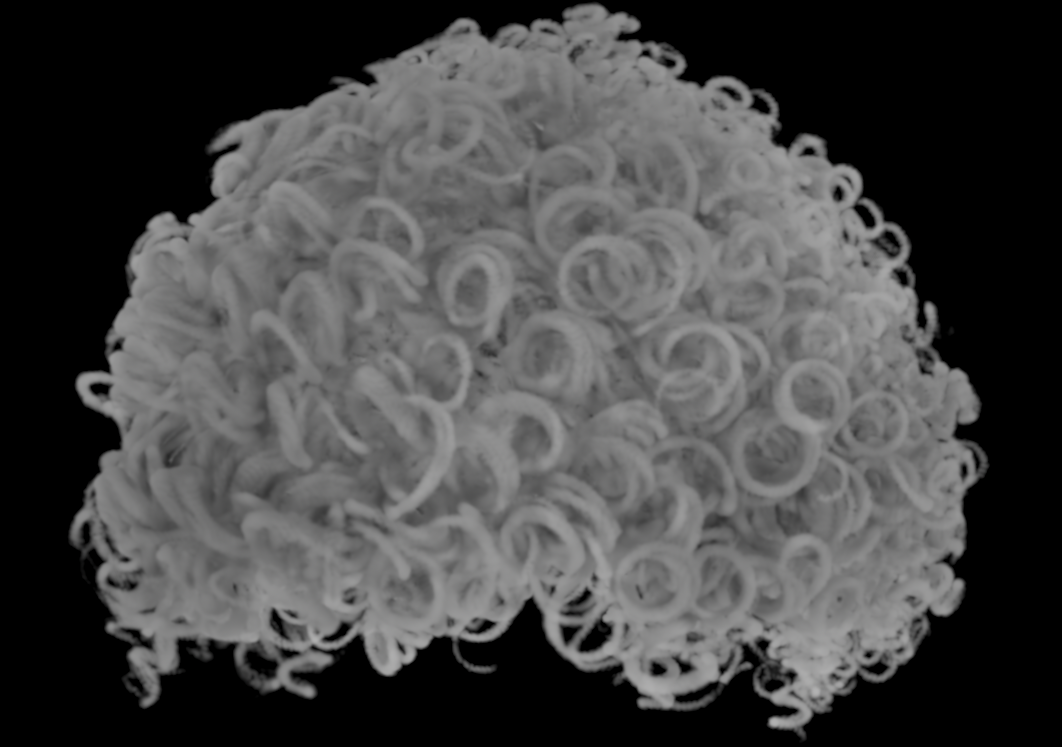
\includegraphics[width=0.5\textwidth]{assets/figures/Screenshot 2025-11-04 135859.png}\hfill
	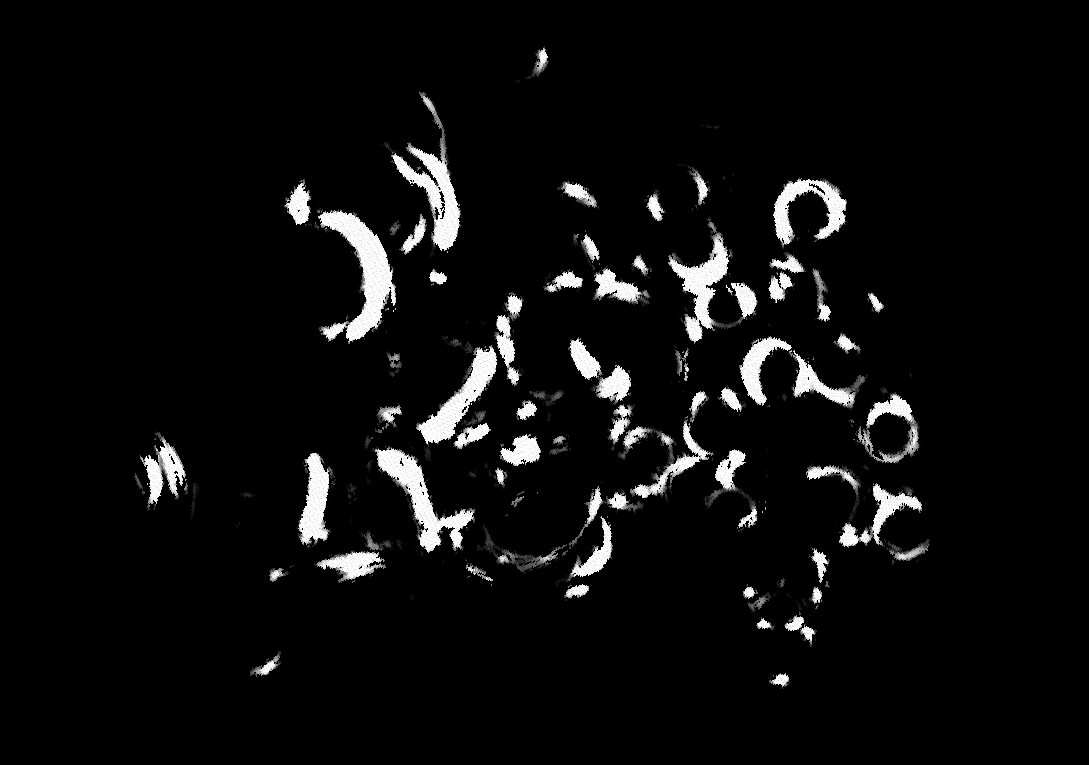
\includegraphics[width=0.5\textwidth]{assets/figures/Screenshot 2025-11-04 140103.png}
	
	\caption{First iteration of the "HairSynth" voxel data base (VDB), point data, and image processing pipeline in Houdini that analyzes hair structure to generate data parameters. These data points are exported via Python script to be used later.}
	\label{fig:hairsynth-iteration1}
\end{figure}

The current technical implementation uses computer vision and image processing to analyze hair structure and gesture in real-time. A rendered video of "slices" from a CT scan of a curly hair "fro" (24 fps for 10 seconds, so 240 slices). A custom python script developed to run in Houdini is used to extract features (a random set of points from the converted VDB to point cloud). These extracted data points are then run through a second python script that converts them to WAV files (at 1024 samples). These are then used in a custom wavetable synthesizer I built in PlugData (an open-source PureData wrapper and VST exporter).

A second version of this uses the program \textit{vvvv} (with built in OpenCV) to extract contour data, key pints, an blobs from the movement patterns of the animated video. These visual features map to synthesis parameters in Max/Msp (like which sample of the wavetable to use). The HairSynth's parameters are scaled and weighted based on the extracted data from the physical properties of hair sample used.

\begin{figure}[htp]
	\centering
	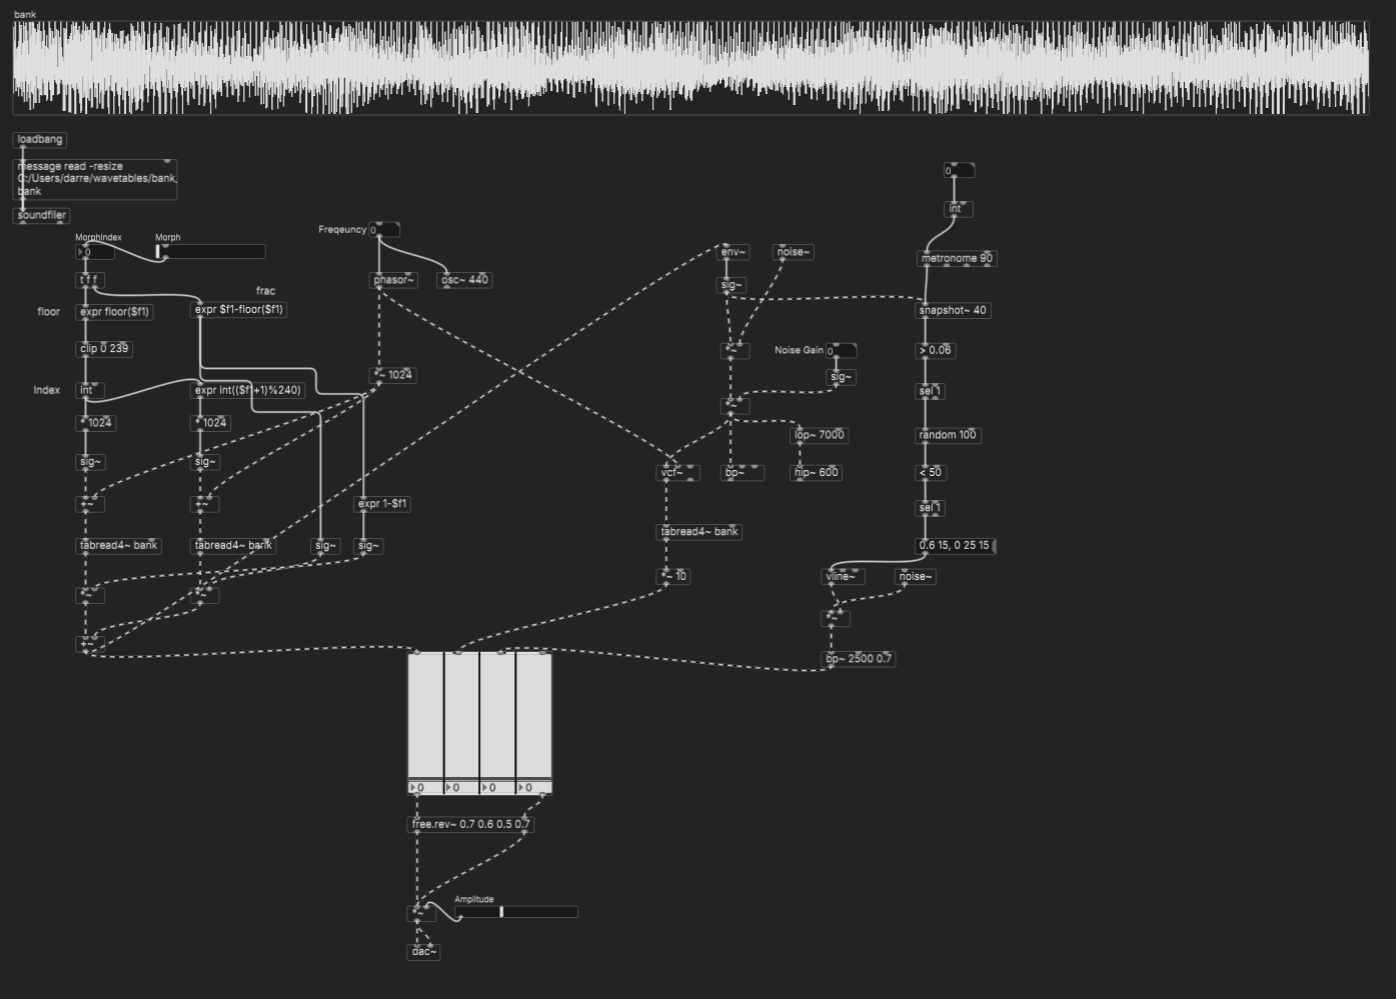
\includegraphics[width=0.75\textwidth]{assets/figures/Screenshot 2025-11-04 141624.png}
	
	\vspace{0.5em}
	
	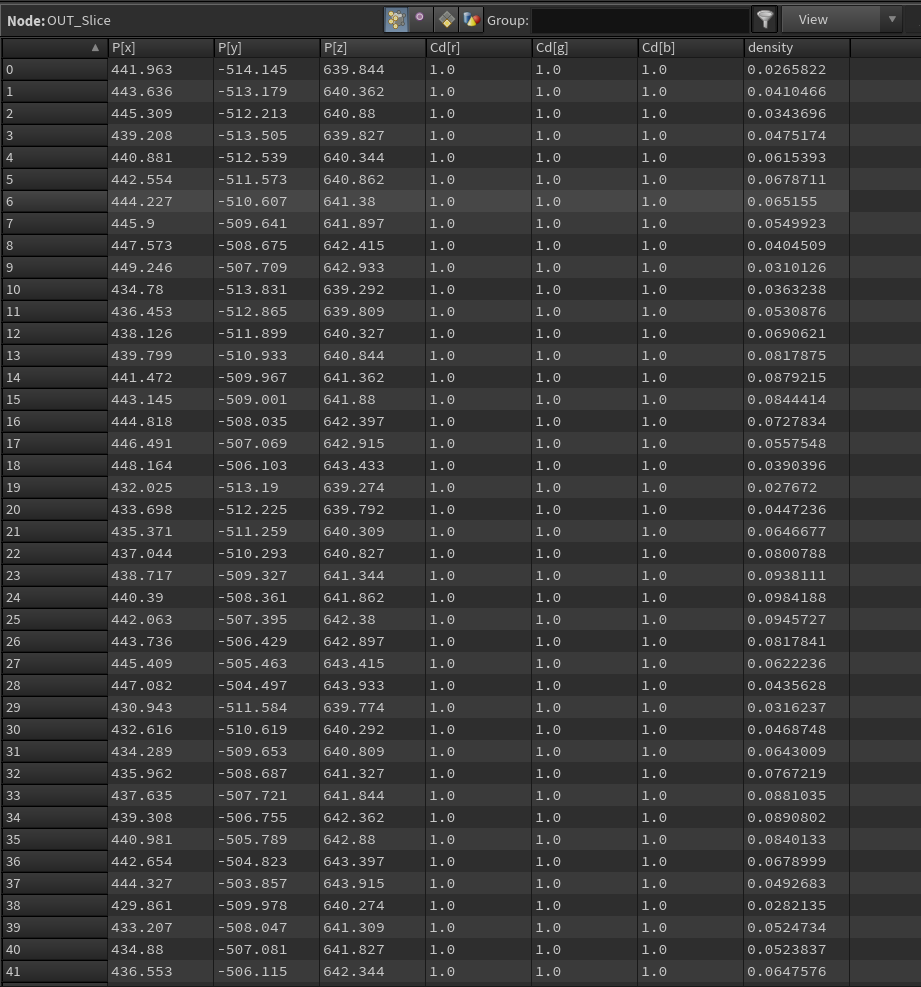
\includegraphics[width=0.5\textwidth]{assets/figures/Screenshot 2025-11-04 140837.png}\hfill
	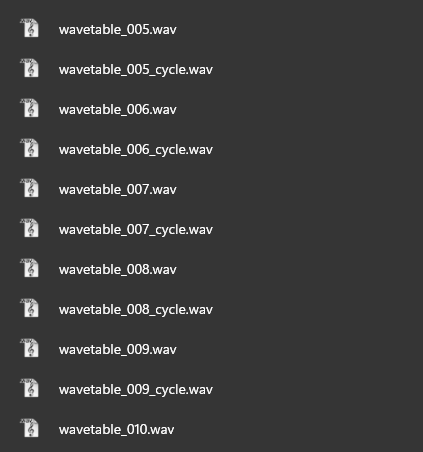
\includegraphics[width=0.5\textwidth]{assets/figures/Screenshot 2025-11-04 141046.png}

	
	\caption{Point data tables, wave (WAV) files, and the subsequent PlugData wavetable synthesizer showing progression of data mapping between extracted hair features and synthesis parameters. The ultimate output of these mappings emerged through embodied experimentation, adjusting values while listening until the sonic output "felt right" in relation to the input and intended sound profile.}
	\label{fig:hairsynth-data}
\end{figure}

The modification work here operates at multiple levels. First, I utilized standard computer vision algorithms (typically designed for facial recognition or object detection) to instead prioritize textural analysis and edge detection at scales appropriate for hair structure. Second, I reconfigured the wavetable synthesis architecture to accept continuous, multidimensional input rather than discrete control messages. Third, I developed a custom extracted hair data-sound mapping system: the synthesizer does not translate "more texture (more values)" into "louder sound" or other simplistic correlations. Instead, the mappings encode relationships informed by my embodied knowledge of my hair. How it feels to touch it, the sounds it makes and when it sound like to get it cut with a "buzzer" or clippers.

The work also includes a visual feedback component where you can see their hair's properties visualized from and animation and extracted features of the slices. I plan to rework and expand this visualization to serve both practical and conceptual functions: practically, it  could help participants understand how the hair drives the synthesis; conceptually, it makes visible the data extraction and quantification processes that the work both employs and critiques.

\subsection{Embodied Development: What Has Emerged}

Working on \emph{Don't Play with My Hair} has been the most technically challenging of the three works, largely because computer vision systems carry deeply embedded assumptions about what bodies look like and how they should be analyzed. Standard algorithms often fail to properly detect or analyze Black hair, particularly natural textures, because training datasets overwhelmingly feature straight, fine hair. In the same vein, there is also a massive lack of what most from an Afro-disaporic background consider their "hair type"(type 4 hair). This first experiment is at best using Type 3 hair in the form of a curly fro. In general, there is a lack of structural" data sets to use for this type of data sonifaction and synthesis. In the future I plan to find ways to use scans and images of my own hair to supplement. This technical friction became a site of unsettling, confronting how even "neutral" image processing tools and development techniques encode racial bias.

The gesture recognition component remains in active development. Currently, the system responds to recorded video, pre-processed to threshold black and white values, but I want to capture more subtle gestures (like gentle touch of fingers running through hair or the twisting of strands), and ultimately, in real-time if possible. These intimate gestures require more sensitive detection and more nuanced mapping strategies. I am exploring whether to add additional sensors (capacitive touch, proximity sensors embedded in headwear) or to refine the vision-based approach further.

\begin{figure}[H]
	\centering
	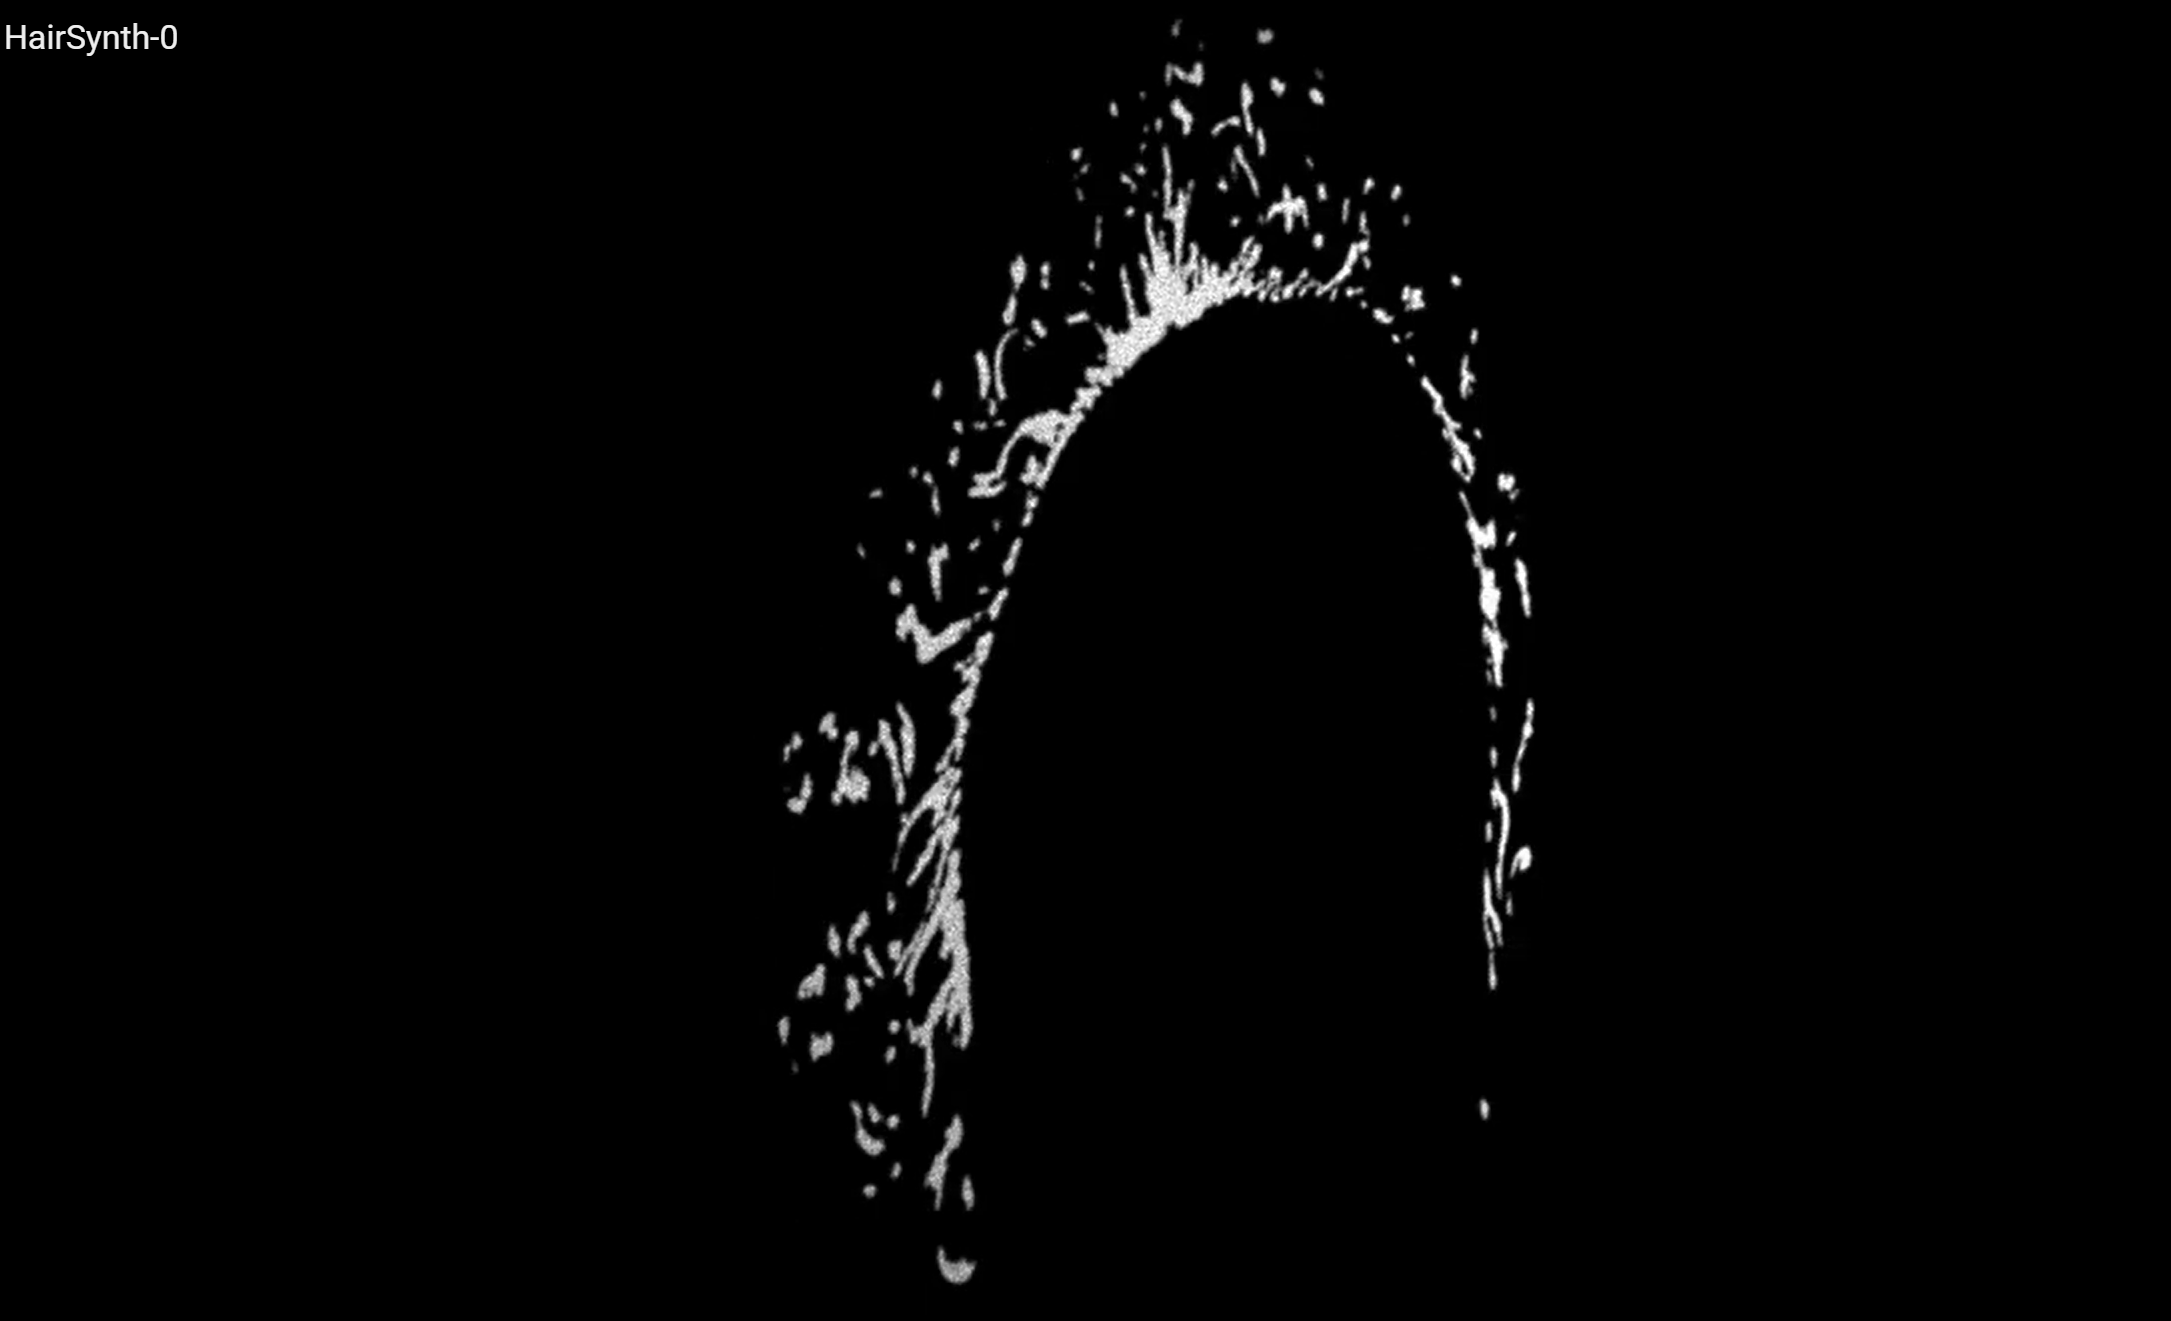
\includegraphics[width=0.75\textwidth]{assets/figures/Screenshot 2025-11-25 181128.png}
	\caption{Still from the 10 second development video showing animation of hair data "slices" and wavetable synth sample. Observe how it is sonically similar to getting hair cur with clippers. [Full video: \url{https://youtu.be/G768Sr5Z_n4}]}
	\label{fig:hairsynth-video}
\end{figure}

The work's framing around consent and boundaries also needs much more development. Initially, I imagined participants would interact with their own hair, maintaining bodily autonomy. But I have been considering whether the work should also allow (with explicit consent protocols) one person to interact with another's hair. The intimacy and the vulnerability of allowing touch that results from this form of interaction. This raises complex questions about how to design consent mechanisms that are not performative but genuinely protective, and whether such interactions risk reproducing the very violations the work critiques.

\subsection{ST Domain Integration}

\textbf{Fugitive Speculation (FS):} The HairSynth refuses the positioning of Black hair as problem to be managed or spectacle to be consumed, instead centering it as a site of knowledge generation and creative agency. By speculating that hair itself can be an instrument, the work imagines technological futures where Black embodiment drives design rather than being accommodated as afterthought.

\textbf{Material Memory (MM):} Hair carries memory in its structure, genetic, environmental, temporal. The choice to use hair structure as synthesis input grounds the work in embodied knowledge of texture, care practices, and the intimate gestures of touching one's own hair. My muscle memory of hair care routines (washing, conditioning, styling) informs the gesture mappings and interaction design.

\textbf{Sensory Worlding (SW):} The work creates a sensory feedback loop between visual (seeing hair, seeing data visualization), tactile (touching hair, feeling gesture), and sonic (hearing synthesis output) modalities. The synthesizer creates a multisensory environment where hair's materiality becomes perceptible across multiple registers simultaneously.

\textbf{Intimate Witnessing (IW):} The work's effectiveness depends on whether the sonic output "feels like" or "sounds-like" hair. Whether the synthesis captures something essential about hair's texture, movement, and intimacy.